\section{Многоуровневая схема редукции размерности с помощью разверток}
\label{sec:multilev_maps}
Одна из постановок задачи глобальной оптимизации звучит следующим образом: найти глобальный минимум \(N\)-мерной функции \(\phi(y)\) в гиперинтервале \(D=\{y\in R^N:a_i\leqslant x_i\leqslant{b_i}, 1\leqslant{i}\leqslant{N}\}\).
Для построения оценки глобального минимума по конечному количеству вычислений значения функции требуется, чтобы \(\phi(y)\) удовлетворяла условию Липшица.
\begin{equation}
\label{task}
\phi(y^*)=\min\{\phi(y):y\in D\}
\end{equation}
\begin{equation}
\label{lip}
|\phi(y_1)-\phi(y_2)|\leqslant L\Vert y_1-y_2\Vert,y_1,y_2\in D,0<L<\infty
\end{equation}
\par
Классической схемой редукции размерности для алгоритмов глобальной оптимизации является использование разверток --- кривых, заполняющих пространство \cite{strSergOptBook}.
\begin{displaymath}
\label{cube}
\lbrace y\in R^N:-2^{-1}\leqslant y_i\leqslant 2^{-1},1\leqslant i\leqslant N\rbrace=\{y(x):0\leqslant x\leqslant 1\}
\end{displaymath}
\par
 Такое отображение позволяет свести задачу в многомерном пространстве к решению одномерной ценой ухудшения её свойств. В частности, одномерная функция \(\phi(y(x))\) является не
 Липшицевой, а Гёльдеровой:
\begin{displaymath}
\label{holder}
|\phi(y(x_1))-\phi(y(x_2))|\leqslant H{|x_1-x_2|}^{\frac{1}{N}},x_1,x_2\in[0,1]
\end{displaymath}
где константа Гельдера \(H\) связана с константой Липшица \(L\) соотношением
\begin{displaymath}
H=4Ld\sqrt{N},d=\max\{b_i-a_i:1\leqslant i\leqslant N\}
\end{displaymath}
\par
Теоретически с помощью этой схемы можно решить задучю любой размерности, однако на ЭВМ развертка строится с помощью конечноразрядной арифметики, из-за чего начиная с некоторого \(N^*\)
построение разветки невозможно (значение \(N^*\) зависит от максимального количества значащих разрядов в арифметике с плавающей точкой).
Понять почему это происходит нетрудно, обратившись, например к \cite{strOptBook}.
\par
Чтобы преодолеть эту проблему профессором В. П. Гергелем была предложена следующая идея: использовать композицию разверток мненьшей размерности для построения отображения
\(z(x): [0;1] \rightarrow D \in R^N\).
Поясним эту схему на примере редукции размерности в четырёхмерной задаче. Пусть \(y_2(x)\) --- двухмертная развертка (отображает отрезок в прямоугольник), тогда рассмотрим функцию
\(\psi(x_1,x_2)=\phi(y_2(x_1), y_2(x_2))\). К \(\psi(x_1,x_2)\) можно также применить редукцию размерности с помощью развертки. Таким образом, задав точку \(x^*\in [0;1]\),
вычислив \(y_2(x^*)=(x_1,x_2)\) и пару векторов \((y_2(x_1), y_2(x_2))\), получим четырёхмерную точку. Из инъективности \(y_2(x)\) следует инъективность \(z(x)\).
\par
Проблемой этого метода является выяснение свойств функции \(\phi(z(x))\) и возможности использования одномерного метода Стронгина с гёльдеровой метрикой для оптимизации \(\phi(z(x))\).
Чтобы не тратить время на теоретическое исследование, были проведены численные эксперименты с целью оценить возможность применения многоуровневой развёртки в четырёхмерном случае.
\par
Прежде всего, рассмотрим линии уровня функции \(\psi(x_1,x_2)=\phi(y_2(x_1), y_2(x_2))\) при \(\phi(t)=\sum_{i=1}^{4}(t_i-0.5)^2\).
\begin{figure}[ht]
	\center
  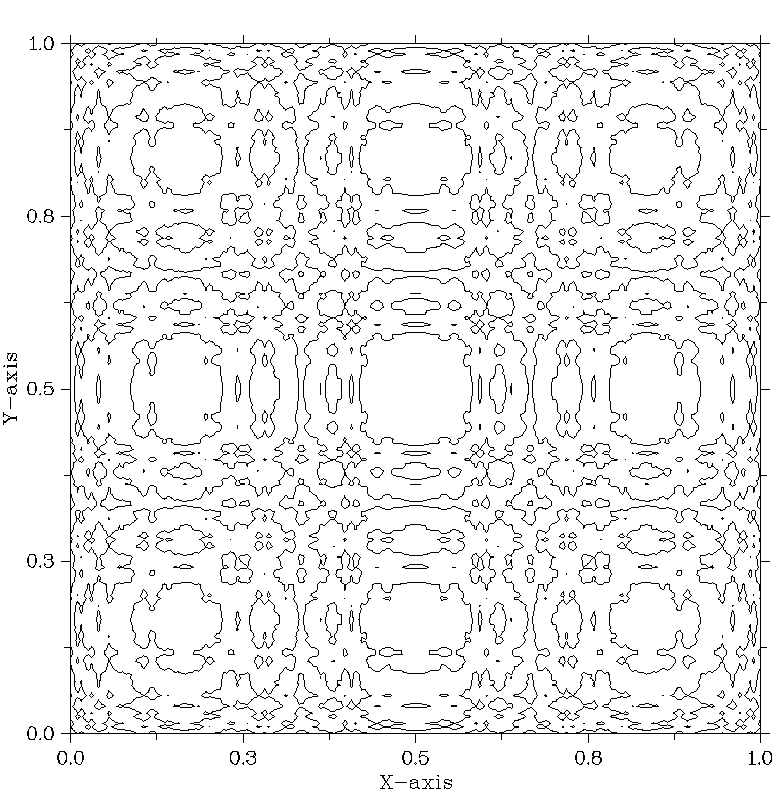
\includegraphics[width=0.55\textwidth]{pictures/multimap_isolines.png}
  \caption{Линии уровня функции \(\psi(x_1,x_2)=\phi(y_2(x_1), y_2(x_2))\)}
  \label{fig:1}
\end{figure}
Как видно из рис. \ref{fig:1}, линии уровня имеют довольно сложную структуру, что говорит о возможных сложностях применения одномерного метода с разверткой.
\par
Далее был проведён более масштабный вычислительный экспеимент: с помощью многоуровневой развертки решались 100 задач из класса GKLS Simple 4d. На рис. \ref{fig:multimapOP} приведены операционные
характеристики метода с простой и многоуровневой развёртками. При этом были зафиксированы следующие параметры алгоритма: надёжность \(r=4.5\), плотность построения всех развёрток 12, критерий остановки попадание
точки, поставленной методом в квадрат со стороной \(\varepsilon=10^{-2}\), центром которого является решение задачи.
\begin{figure}[ht]
	\center
  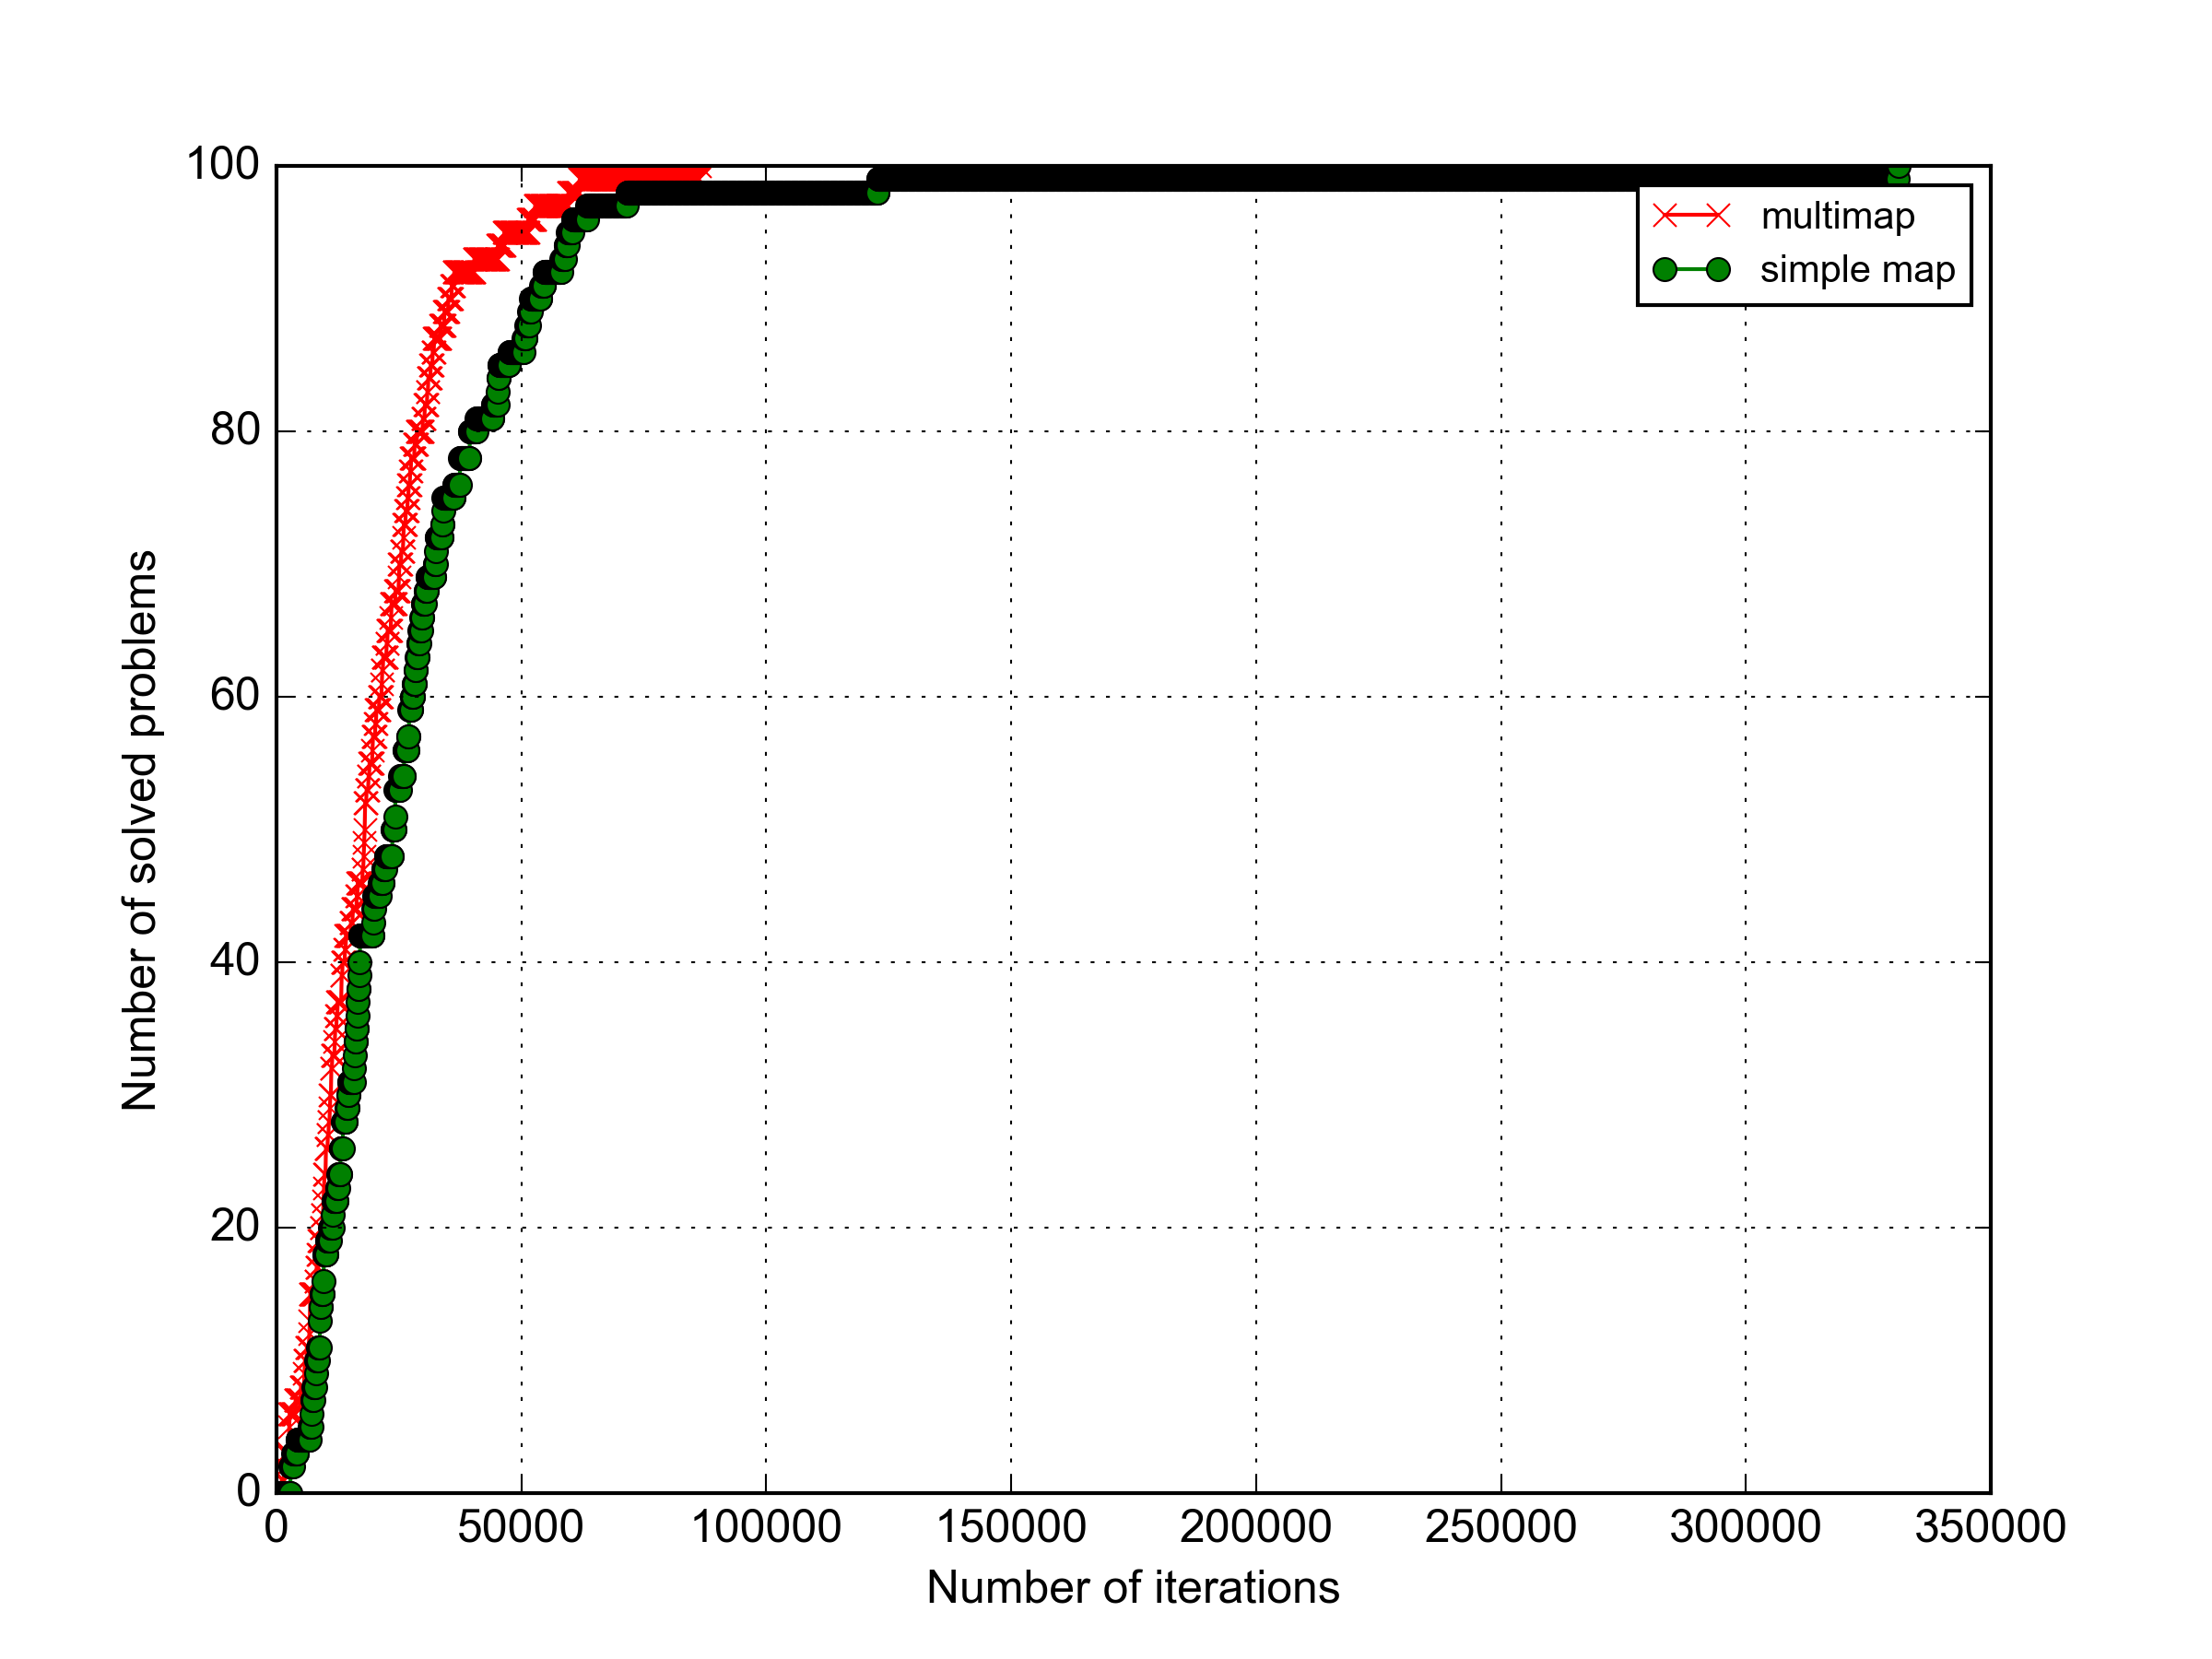
\includegraphics[width=0.75\textwidth]{pictures/multimap_op.png}
  \caption{Операционная характеристика метода с различными развёртками на классе GKLS Simple 4d}
  \label{fig:multimapOP}
\end{figure}
Как видно из графика, операционная характеристика метода с многоуровневой развёрткой лежит выше, чем аналогичная кривая метода с простой развёрткой. Кроме того, метод с многоуровневой развёрткой
заметно раньше вышел на стопроцентную надёжность на решаемой выборке задач. Исходя из первых экспериментов можно сказать, что при данных параметрах алгоритма многоуровневая развертка лучше, но
при уменьшении точности алгоритма \(\varepsilon\) до значения \(10^{-3}\) выполнения критерия остановки в случае использования многоуровневой развёртки с выбранной плотностью построения внутренних развёрток не происходит.
Если плотность увеличить до 16, то остановка также не будет происходить. Исходя из этого можно делать вывод, что использование на практике многоуровневых развёрток с большой долей вероятности
невозможно из-за описанного дефекта сходимости.
